\documentclass{article}

\usepackage{amsmath}
\usepackage{graphicx}
\usepackage{subcaption}
\usepackage{setspace}
\usepackage[backend=bibtex]{biblatex}

\bibliography{test}

% Preable section
\title{My first document}
\date{2020-04-11}
\author{Alexander Baquiax}
\setcounter{tocdepth}{3} % 3 shos subsections


\begin{document}

\pagenumbering{gobble}

\maketitle
\newpage

\doublespacing
\tableofcontents
\singlespacing
\newpage

\pagenumbering{arabic}



\section{Section}
Structuring a document is easy!

\subsection{Subsection}
More text.

\paragraph{Paragraph}
Some more text.

\subparagraph{Subparagraph 1}
Even more text.

\section{Another section}

Here a simple equation:

Here a simple equation without number:
\begin{equation*}
    f(x) = x*x
\end{equation*}

\begin{equation}
    f(x) = x^2
\end{equation}

In text you can also include a formula wrapping it in dollar symbols e.g $a^2$

\section{Math}
You can add equations with an environment as well.
\begin{equation}
    A = Z + 2
\end{equation}

If you have a expression with multiple equations you can align them

\begin{align}
    A + 1 & = 2     \\ % Is like a \n
    B + A & = 3 + 1 % The & before the = represent the point to align
\end{align}

\subsection{More math expressions}
\begin{align*}
    f(x) & = x^2                     \\
    g(x) & = \frac{1}{x}             \\
    F(x) & = \int^a_b \frac{1}{3}x^3 \\
\end{align*}

\begin{equation*}
    \frac{1}{\sqrt{x}}
\end{equation*}

\section{Matrices}

\begin{equation}
    \begin{matrix}
        1 & 0 \\
        0 & 1
    \end{matrix}
\end{equation}

\begin{equation}
    \left[
        \begin{matrix}
            1 & 0 \\
            0 & 1
        \end{matrix}
        \right]
    \left(\sqrt{1} + 2\right)
\end{equation}

\section{Figures}

\begin{figure}[h] % h means: here
    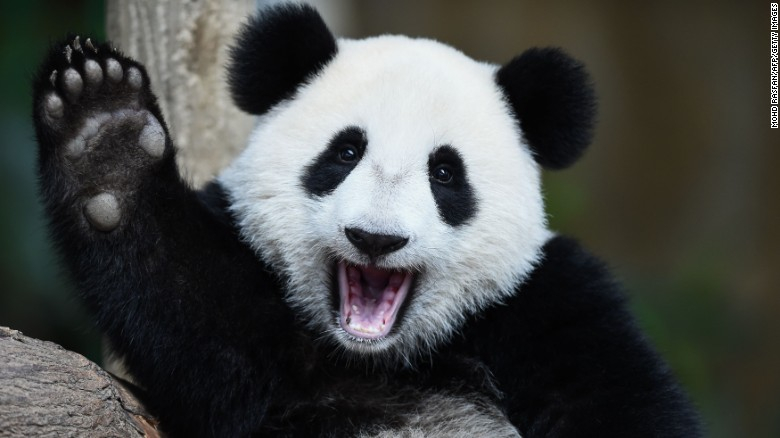
\includegraphics[width=\linewidth]{images/panda.jpg}
    \caption{A panda.}
    \label{fig:panda}
\end{figure}


\begin{figure}[h!]
    \centering
    \begin{subfigure}[b]{0.4\linewidth} % b = bottom and 0.4 means 40% of the page width
        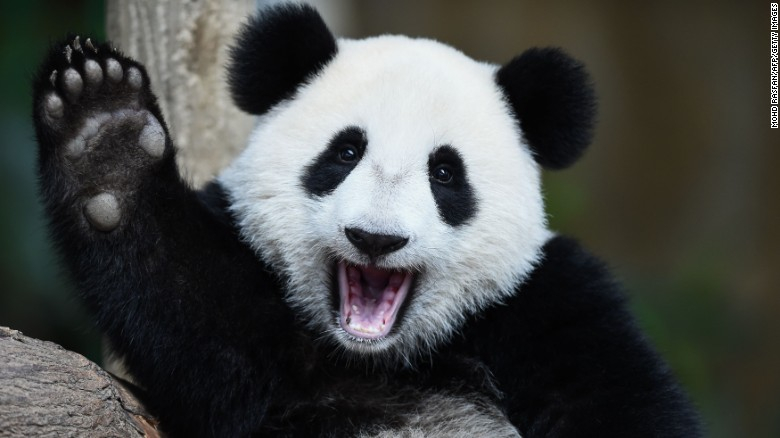
\includegraphics[width=\linewidth]{images/panda.jpg}
        \caption{Pandita}
    \end{subfigure}
    \begin{subfigure}[b]{0.4\linewidth}
        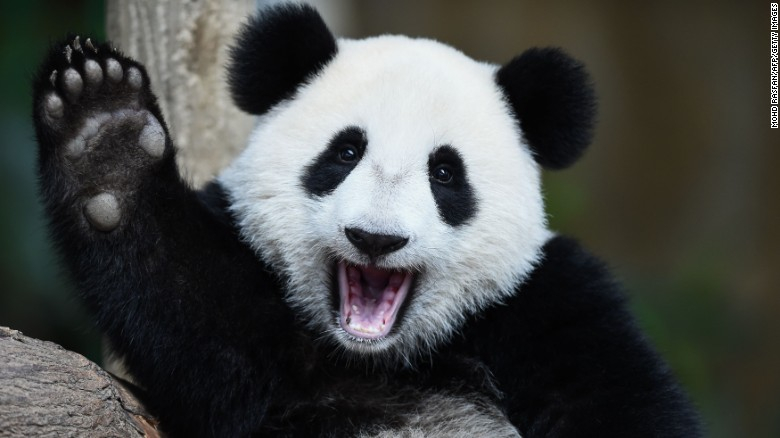
\includegraphics[width=\linewidth]{images/panda.jpg}
        \caption{Other pandita}
    \end{subfigure}
    \caption{A pair of good pandas}
\end{figure}

\section{Tables}

\begin{table}
    \caption{A dummy table}
\end{table}

\section{Cite}
Random citation \autocite{DUMMY:1} embedded in text.

\newpage
This is a footnote \footnote{\label{myFootNote} Hello}

Im refering to \ref{myFootNote}
\newpage

\printbibliography

\begin{appendix}
    \listoffigures
    \listoftables
\end{appendix}
\newpage

\end{document}
